\section{Introduction}

Advanced extracellular recording technologies now enable neuroscientists to capture unprecedented volumes of high-dimensional neural\footnote{By default, "neural" and "neuron" will refer to neurobiology; e.g. we may call biological neuronal spike data "neural activity". In contrast, activity and neurons from artificial neural networks will be explicitly prefaced; e.g. "artificial neural activity" or "the model's neurons".} data at single-cell resolution ~\cite{steinmetz_2021_neuropixels2, raducanu_2017_neuroseeker, cai_2016_miniscope, villette_2019_voltage_2p, ouzounov_2017_three_photon, ahrens_2013_lightsheet}. Understanding the computational principles driving neural activity requires extracting interpretable features from this data. Traditional dimensionality reduction techniques, while useful for visualization and basic analyses, often make invalid assumptions about or altogether fail to disentangle distributed representations, and as a result typically cannot provide a mechanistic understanding of the underlying computations ~\cite{cunningham_2014_neural_dr, humphries_2021_dr_principles}. Recent work has produced promising latent variable model (LVM) approaches capable of identifying low-dimensional subspaces that can accurately decode aspects of behavior and environment ~\cite{song_2025_langevinflow, schneider_2023_cebra, le_2022_stndt, keshtkaran_2022_autolfads, yu_2009_gpfa, macke_2011_plds, gao_2016_pflds, low_2018_mind, jensen_2020_mgplvm, hernandez_2020_vind, kim_2021_plnde, hurwitz_2021_tndm, schimel_2022_ilqrvae, kudryashova_2023_ctrltndm, ye_2023_ndt2, gondur_2024_mmgpvae, pellegrino_2024_slicetca, sani_2024_dpad, pals_2024_smclr_rnn, zhang_2024_mtm, george_2025_simpl, perkins_2025_mint, schmutz_2025_nce}. However, these methods typically value decoding accuracy over latent interpretability, and consequently all have at least one of the following limitations: poorly interpretable latents, lossy mapping to and/or poor reconstruction of neural data from latent space, priors on the latent and/or neural data space, requirements of additional behavioral, environmental, and/or trial-structured neural data, supralinear scaling with respect to dataset size, or high implementational complexity.

We address each of these limitations in MINI, which provides a simple, user-friendly library for interpretable latent discovery from high-dimensional neural data. We consider a latent's interpretability in two key aspects: 1) its correspondence to a specific external variable -- a "natural" behavioral or environmental feature\footnote{A "feature" is a sufficiently interpretable latent. We illustrate this in \nameref{section:results}.}; 2) its explicit composition from contributing neural activity. MINI's approach obviates the need for post-hoc analyses to find meaningful dynamics in latent spaces typical of other approaches. Additionally, while we showcase MINI on spike data, it can be readily used with virtually any other neural recording modality as the only data requirement is any predefined spatiotemporal binning.

At MINI's core is the training of shallow sparse dictionary neural network (SDNN) models whose individual dictionary elements -- hidden layer neurons -- ideally serve as interpretable latents. This particular LVM approach has had many successes in the field of AI mechanistic interpretability ~\cite{cunningham_2023_saes, bricken_2023_towards_monosemanticity, templeton_2024_scaling_monosemanticity, ameisen_2025_circuit_tracing, lindsey_2025_biology_llm}, and here is additionally motivated by the principle that we need not explicitly impose structure on the latent space nor model its dynamics to discover interpretable variables. Specifically, MINI bypasses the need to enforce non-Markovian dynamics, which are often a property of an incomplete observation of a system rather than the system itself; any dynamical system can be represented as Markovian via sufficient state augmentation ~\cite{takens_1981_embedding}. Given this, even methods that appear non-Markovian can be seen as attempts to approximate a complete underlying state. For example, the forward dynamics of a recurrent neural network (RNN) are Markovian in its hidden state ~\cite{sussillo_2013_rnn_dynamics, goodfellow_2016_rnn}, and generalized linear models (GLMs) with history filters ~\cite{pillow_2008_glms, truccolo_2005_pointprocess} use past activity to augment the present state. This perspective aligns with several findings in neuroscience, from activity in motor cortex reflecting a low-dimensional, implicitly Markovian dynamical system ~\cite{churchland_2012_population_dynamics, shenoy_2013_dynamical_perspective}, to predictive-coding formulations that posit that the brain maintains an internal state sufficient to predict sensory streams, i.e., a Markovian latent process \cite{rao_1999_predictive_coding, doya_2007_bayesian_brain, friston_2010_free_energy}. Grounded in this perspective, MINI forgoes the challenge of modeling intricate dynamics and instead directly extracts meaningful constituent features of the underlying neural state (\autoref{figure:interpretable_latents_vs_latent_space}).

\begin{figure}[h]
    \label{figure:interpretable_latents_vs_latent_space}
    \centering
    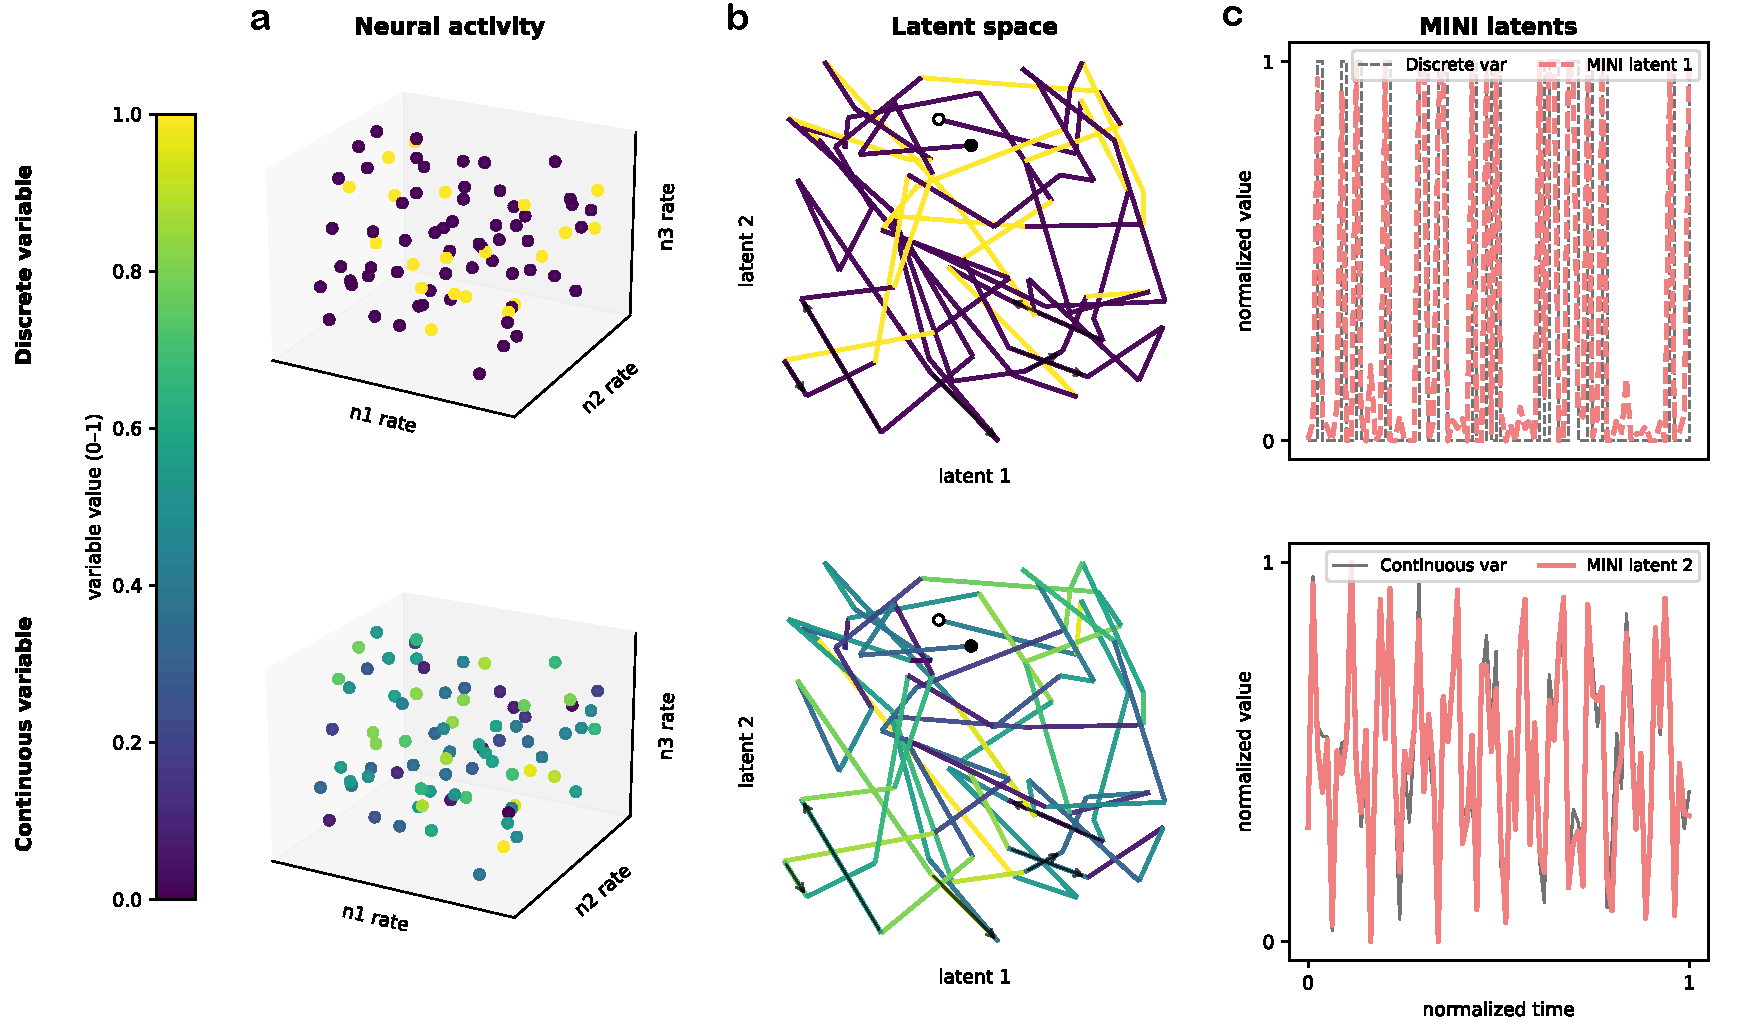
\includegraphics[width=\linewidth]{figures/interpretable_latents_vs_latent_space.pdf}
    \caption{
        \textbf{Interpretable latents vs. latent space.} \\
        \small This toy example highlights the utility of MINI. The two rows show two different variables (top: discrete; bottom: continuous), each uniquely encoded by the same underlying neural activity made up of three neurons' firing rates. The viridis colorbar shows the variables' values as a function of this neural activity. (\textbf{a}) Each point in the scatterplots represents a moment in time. (\textbf{b}) A projection of this activity into a 2D latent space creates tangled trajectories where variable states (e.g. 'on' and 'off' in the discrete case, and 'high' and 'low' in the continuous case) are not easily distnguished. The start and end points of the trajectories are marked by white and black dots, respectively, while arrows indicate trajectory direction. (\textbf{c}) In contrast to the tangled latent space, MINI finds individual latents corresponding to each variable, demonstrating the potential for improved interpretability of neural representations.
    }
\end{figure}